\section{Общие сведения об объекте автоматизации}

Система управляющей компании жилого дома предназначена для организации и учёта плановых ремонтных работ и внеплановых заявок на проведение работ от жильцов.

В плановые мероприятия в первую очередь входят содержание дома и технический надзор:
\begin{itemize}
\item санитарная уборка общего помещения подъезда и первых 4-х этажей дома (1 раз в день)
\item санитарная уборка верхних этажей (1 раз в неделю)
\item осмотр магистральных водопроводных коммуникаций (2 раза в день)
\item осмотр технических магистральных коммуникаций (электрическая проводка, интернет, телефонная связь)
\item обследования крыш, чердаков, подъездов, фасадов, внешнего благоустройства (не реже 1 раза в 2 дня)
\item уборка придомовой территории (1 раз в день)
\end{itemize}

Так же в плановые мероприятия входит подготовка к сезонной эксплуатации:

\begin{itemize}
\item обследование и уборка снега и льда с крыш (ежедневно с ноября по март)
\item полное инженерное обследование магистральных труб горячей воды (1 раз летом, длительностью не дольше недели)
\end{itemize}
В случае обнаружения компанией неисправностей или нарушений работоспособностей конструкций, инженерного оборудования в поднадзорных УК помещений, компании надлежит провести немедленный ремонт.

Иные работы в поднадзорных УК помещениях или в помещениях жилых квартир проводятся по заказам и за счёт средств потребителей. 

Перечисленные работы выполняются следующими функциональными бригадами (каждая имеет две смены):
\begin{itemize}
\item Сантехники (работы по водопроводному оборудованию)
\item Электрики (работы с электрикой, телефонной и интернет связью)
\item Уборщики (санитарная уборка общедомового помещения, придомовой территории и фасадов
\item Инженеры (поддержание работоспособности и исправности конструкций дома)
\end{itemize}

Деятельность УК включает следующие функции:
\begin{enumerate}
\item Глава УК и бригадиры формируют расписание плановых работ по жилому дому
\item Жильцы подают заявки на проведение заказных работ - за час и ранее до ориентировочного начала выполнения задачи он может отменить заявку
\item Диспетчер распределяет все задачи по сменам и задаёт порядок их выполнения 
\item Сотрудники бригад в установленном порядке выполняют задачи и объявляют об их выполнении
\item Бригадиры утверждают выполненный статус задачи
\item Диспетчер снимает задачу и уведомляет о выполненном заказе жильца
\end{enumerate}

\section{Требования к функциям системы}

\begin{enumerate}
\item Система должна позволять вести следующие справочники и классификаторы:
\begin{itemize}
\item Справочник сотрудников
\item Справочник зарегистрированных в системе жильцов дома
\item Квартиры в доме
\item Бригады
\item Архив задач
\end{itemize}
\item Система должна обеспечивать выполнение следующих функции:
\begin{itemize}
\item Формирование списка невыполненных заявок в реальном времени
\item Назначение сотрудников в равной степени на невыполненные задачи 
\item Изменение назначений исполнителя работ бригадирами
\item Формирование отчёта о выполненной заявке
\end{itemize}
\end{enumerate}


\section{Приложение к пунктам 1.3-1.4}

\begin{figure}[h]
\centering
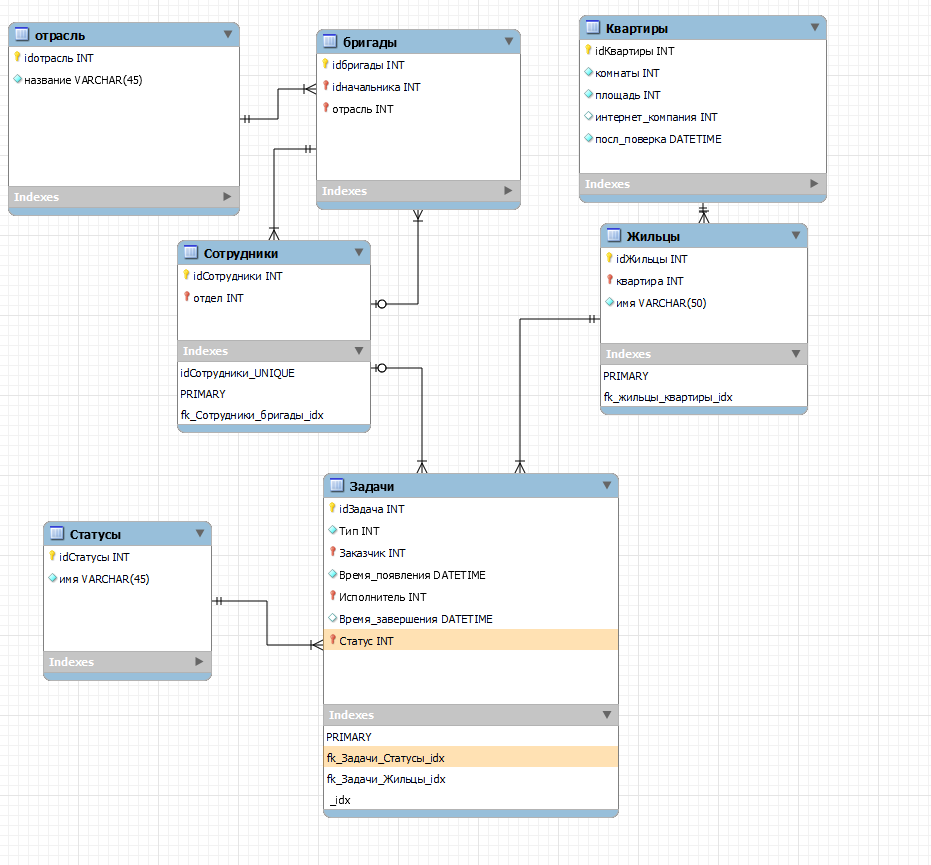
\includegraphics[width=0.7\textwidth]{Images/model.png}
\caption{ER-диаграмма модели базы данных}
\end{figure}


\begin{figure}[h]
\centering
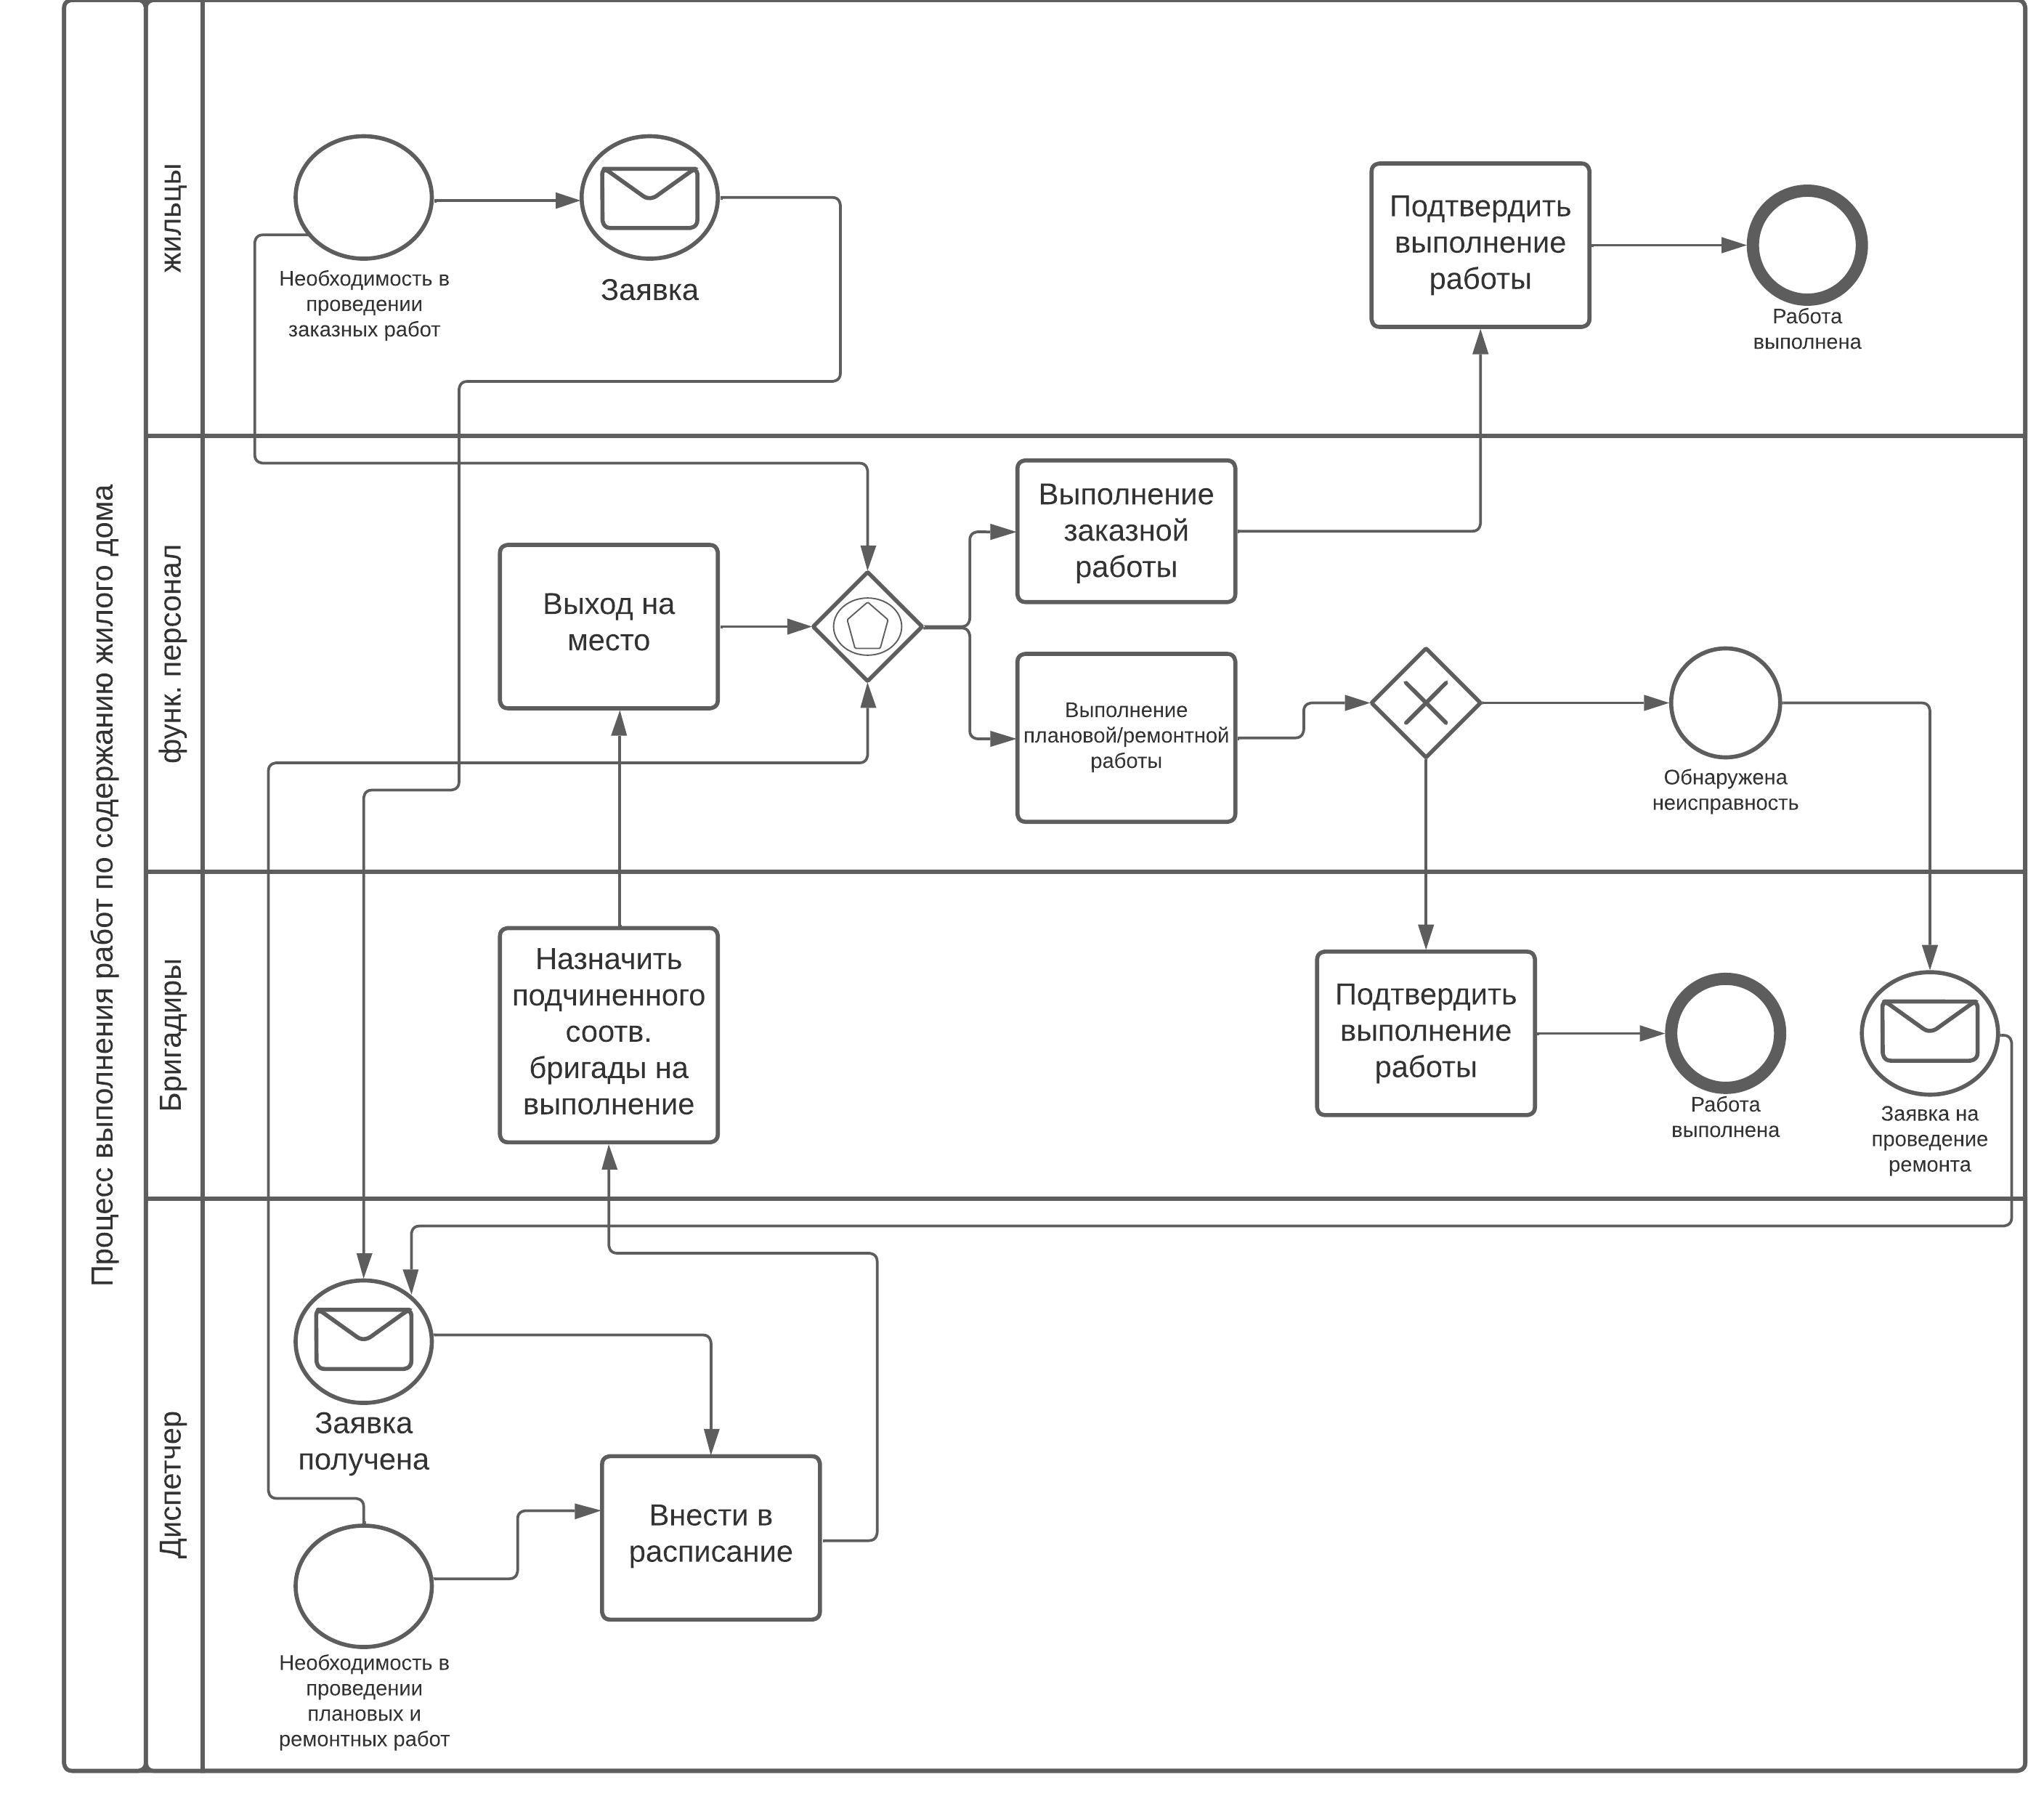
\includegraphics[width=0.7\textwidth]{Images/process.png}
\caption{Модель процессов, автоматизируемых с помощью Системы в нотации BPMN}
\end{figure}


\begin{figure}[h]
\centering
\includegraphics[width=0.7\textwidth]{Images/interface.png}
\caption{Набросок интерфейса системы}
\end{figure}


\s
 